\begin{figure}
\begin{minipage}{6in}
\begin{center}

\begin{subfigure}[b]{0.45\columnwidth}
\centering
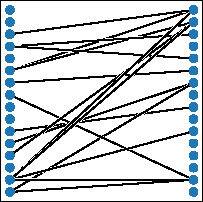
\includegraphics[width=\textwidth]{graph_layouts/title=irregular-1+ext=}%
\caption{
Irregular configuration with mean degree 1
}
\label{fig:irregular_1}
\end{subfigure}
\begin{subfigure}[b]{0.45\columnwidth}
\centering
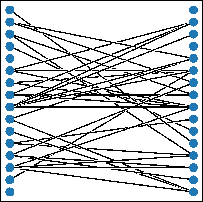
\includegraphics[width=\textwidth]{graph_layouts/title=irregular-2+ext=}%
\caption{
Irregular configuration with mean degree 2
}
\label{fig:irregular_2}
\end{subfigure}

\begin{subfigure}[b]{0.45\columnwidth}
\centering
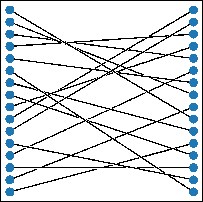
\includegraphics[width=\textwidth]{graph_layouts/title=regular-1+ext=}%
\caption{
Regular configuration with mean degree 1
}
\label{fig:regular_1}
\end{subfigure}
\begin{subfigure}[b]{0.44\columnwidth}
\centering
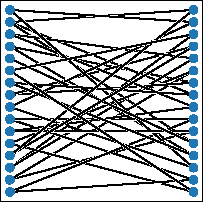
\includegraphics[width=\textwidth]{graph_layouts/title=regular-2+ext=}%
\caption{
Regular configuration with mean degree 2
}
\label{fig:regular_2}
\end{subfigure}

\caption{
Depiction of the target graph layouts used in evolutionary experiments.
}
\label{fig:graph_layouts}

\end{center}
\end{minipage}
\end{figure}
